\documentclass[color=usenames,dvipsnames]{beamer}\usepackage[]{graphicx}\usepackage[]{color}
% maxwidth is the original width if it is less than linewidth
% otherwise use linewidth (to make sure the graphics do not exceed the margin)
\makeatletter
\def\maxwidth{ %
  \ifdim\Gin@nat@width>\linewidth
    \linewidth
  \else
    \Gin@nat@width
  \fi
}
\makeatother

\definecolor{fgcolor}{rgb}{0.345, 0.345, 0.345}
\newcommand{\hlnum}[1]{\textcolor[rgb]{0.686,0.059,0.569}{#1}}%
\newcommand{\hlstr}[1]{\textcolor[rgb]{0.192,0.494,0.8}{#1}}%
\newcommand{\hlcom}[1]{\textcolor[rgb]{0.678,0.584,0.686}{\textit{#1}}}%
\newcommand{\hlopt}[1]{\textcolor[rgb]{0,0,0}{#1}}%
\newcommand{\hlstd}[1]{\textcolor[rgb]{0.345,0.345,0.345}{#1}}%
\newcommand{\hlkwa}[1]{\textcolor[rgb]{0.161,0.373,0.58}{\textbf{#1}}}%
\newcommand{\hlkwb}[1]{\textcolor[rgb]{0.69,0.353,0.396}{#1}}%
\newcommand{\hlkwc}[1]{\textcolor[rgb]{0.333,0.667,0.333}{#1}}%
\newcommand{\hlkwd}[1]{\textcolor[rgb]{0.737,0.353,0.396}{\textbf{#1}}}%
\let\hlipl\hlkwb

\usepackage{framed}
\makeatletter
\newenvironment{kframe}{%
 \def\at@end@of@kframe{}%
 \ifinner\ifhmode%
  \def\at@end@of@kframe{\end{minipage}}%
  \begin{minipage}{\columnwidth}%
 \fi\fi%
 \def\FrameCommand##1{\hskip\@totalleftmargin \hskip-\fboxsep
 \colorbox{shadecolor}{##1}\hskip-\fboxsep
     % There is no \\@totalrightmargin, so:
     \hskip-\linewidth \hskip-\@totalleftmargin \hskip\columnwidth}%
 \MakeFramed {\advance\hsize-\width
   \@totalleftmargin\z@ \linewidth\hsize
   \@setminipage}}%
 {\par\unskip\endMakeFramed%
 \at@end@of@kframe}
\makeatother

\definecolor{shadecolor}{rgb}{.97, .97, .97}
\definecolor{messagecolor}{rgb}{0, 0, 0}
\definecolor{warningcolor}{rgb}{1, 0, 1}
\definecolor{errorcolor}{rgb}{1, 0, 0}
\newenvironment{knitrout}{}{} % an empty environment to be redefined in TeX

\usepackage{alltt}
%\documentclass[color=usenames,dvipsnames,handout]{beamer}

%\usepackage[roman]{../pres1}
\usepackage[sans]{../pres1}

%\usepackage{changepage}


%\newcommand{\wide}{\column{\dimexpr\paperwidth}} % Must be in columns environment




\IfFileExists{upquote.sty}{\usepackage{upquote}}{}
\begin{document}

\begin{frame}[plain]
  \begin{center}
    {\huge Harvest Models} \\
%    {\large January 28 \& 30, 2019} \\
    \vfill
    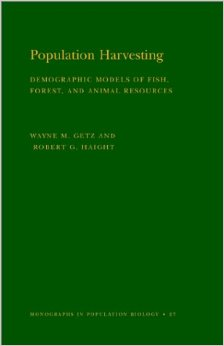
\includegraphics[height=5.5cm,keepaspectratio]{figs/book} \hspace{0.3cm}
    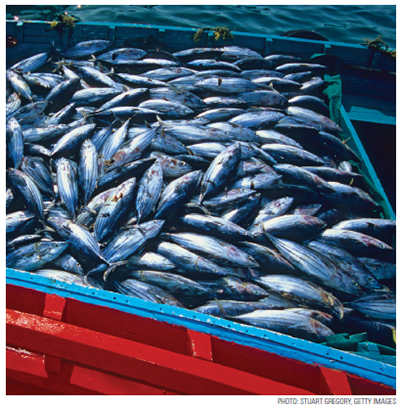
\includegraphics[height=5.5cm,keepaspectratio]{figs/tuna}
  \end{center}
\end{frame}

% QUIZ: Write down and label (1) exponential growth and (2) logistic growth


\begin{frame}
  \frametitle{Today's topics}
  \large
%  \begin{itemize}
%  \item
  Sustainable harvest and geometric growth \\
  \vfill
  % \item
  Sustainable harvest and logistic growth \\
  \vfill
  % \item
  Definition of maximum sustainable yield (MSY) \\
  \vfill
  % \item
  Limitations of MSY \\
  \vfill
  % \item
  Additive vs compensatory mortality
%    \item Definition of compensatory mortality
%  \end{itemize}
\end{frame}


%\section{Introduction}



%% \begin{frame}
%%   \frametitle{Harvest}
%% How is it that we can harvest 2M ducks each year and the population
%% size doesn't change much?

%% How is it that cats can kill 2M songbirds each year and the population
%% size doesn't change much?

%% \end{frame}





\begin{frame}
  \frametitle{Sustainable harvest}
  \large
  {%\bf
    A sustainable (and large) harvest is a common
    objective in game management}
  \vfill
  \pause
%  \begin{block}{Definition}
  {%\bf
    Sustainable harvest:}
    A harvest that is balanced by population growth such that $N_{t+1}
    = N_t$
%  \end{block}
\end{frame}





\section{Geometric growth}




\begin{frame}
  \frametitle{Harvest and geometric growth}
  \Large
  \[
   N_{t+1} = N_t + N_tr \pause - \color{red}{H_t}
  \] \\
  \pause
%  \vspace{1cm}
  \large
  where $H_t$ is the number of animals harvested at the end of year $t$ \\
  \pause
  \vfill %\vspace{2cm}
%  \Large
%  \vfill
  What value of $H_t$ achieves equilibrium (i.e., $N_{t+1} = N_t$)?  \\
%  \pause
%  \vfill
%  Equilibrium is condition in which $N_{t+1} = N_t$?
\end{frame}




\begin{frame}
  \frametitle{Sustainable harvest and geometric growth}
  \large
  A sustainable harvest in this context is
  \LARGE
  \[
    H_t = N_tr
  \]
  \pause
  \large
  \vfill
  {%\centering
    Consequently, the sustainbale harvest rate ($h$) is: \par}
  \LARGE
  % \[
  %   h = \frac{H_t}{N_t} = r
  % \]
  \begin{align*}
    h &= \frac{H_t}{N_t} \\
    \uncover<3->{h}  &\uncover<3->{= r} \\
  \end{align*}
\end{frame}





\section{Logistic growth}


%% \begin{frame}[fragile]
%%   \frametitle{Harvest and logistic growth}
%%     The ``doomed surplus''
%%     \vspace{-0.8cm}
%%   \begin{center}
%% <<logistic1,fig=TRUE,include=FALSE,echo=FALSE>>=
%% T <- 100
%% Ne <- Np <- Nl <- integer(T-1)
%% rmax <- 0.1
%% K <- 1000
%% Ne[1] <- Np <- Nl[1] <- 1
%% for(t in 1:T) {
%%     Ne[t+1] <- Ne[t] + Ne[t]*rmax
%%     Nl[t+1] <- Nl[t] + Nl[t]*rmax*(1 - Nl[t]/K)
%%     Np[t+1] <- Nl[t] + Nl[t]*rmax
%%     }
%% plot(0:T, Np, type="l", col="blue", lwd=3,
%%      ylab="Population size",
%%      xlab="Time", las=2, cex.lab=1.5)
%% lines(0:T, Nl, lwd=2)
%% #polygon(c(0:T, T:0), c(Nl, rev(Ne)), density=100, col=gray(0.7))
%% legend(0, 14000, c("Geometric (potential) growth",
%%                    "Logistic growth"),
%%        lwd=2, col=c("blue", "black"))

%% @
%% <<logistic2,fig=TRUE,include=FALSE,echo=FALSE>>=
%% T <- 100
%% Ne <- Nl <- integer(T-1)
%% rmax <- 0.1
%% K <- 1000
%% Ne[1] <- Nl[1] <- 1
%% for(t in 1:T) {
%%     Ne[t+1] <- Ne[t] + Ne[t]*rmax
%%     Nl[t+1] <- Nl[t] + Nl[t]*rmax*(1 - Nl[t]/K)
%%     }
%% plot(0:T, Ne, type="l", col="blue", lwd=2,
%%      ylab="Population size",
%%      xlab="Time", las=2, cex.lab=1.5)
%% lines(0:T, Nl, lwd=2)
%% polygon(c(0:T, T:0), c(Nl, rev(Ne)), density=100, col=gray(0.7))
%% legend(0, 14000, c("Geometric (potential) growth",
%%                    "Logistic growth"),
%%        lwd=2, col=c("blue", "black"))
%% @
%% %  \only<1>{\includegraphics[fig.width=0.8\textwidth]{harvest-logistic1}}
%% %  \only<2>{\includegraphics[fig.width=0.8\textwidth]{harvest-logistic2}}
%%   \includegraphics[fig.width=0.8\textwidth]{harvest-logistic2}
%% \end{center}
%% \end{frame}




\begin{frame}
  \frametitle{Harvest and logistic growth}
  \LARGE
  \[
    N_{t+1} = N_t + N_t r_{max}\left(1 - \frac{N_t}{K} \right) - \alert{H_t}
  \]
  \pause
%  \vspace{2cm}
  \vfill
  \Large
  \centering %\bf
  What value of $H_t$ achieves equilibrium? \\
\end{frame}



\begin{frame}
  \frametitle{Sustainable harvest and logistic growth}
  \LARGE
  \[
    H_t = N_t r_{max}\left(1 - \frac{N_t}{K} \right)
  \]
  \pause
  \vfill
  \Large
%  \bf
  In this case, the sustainable harvest rate ($h$) depends on population size
  \vfill
  \pause
  % \[
  %   h_t = \frac{H_t}{N_t} = r_{max}\left(1 - \frac{N_t}{K} \right)
  % \]
  \begin{align*}
    h_t &= \frac{H_t}{N_t} \\
    \uncover<4->{h_t &= r_{max}\left(1 - \frac{N_t}{K} \right)} \\
  \end{align*}
\end{frame}



\begin{frame}[fragile]
  \frametitle{Example when $K=1000$ and $r_{max}=0.1$}
  \scriptsize
  \[
    H_t = N_t r_{max}\left(1 - \frac{N_t}{K} \right)
  \]
  \vspace{-1cm}
%<<msy1,fig=TRUE,include=FALSE,fig.width=12,fig.height=6,echo=FALSE>>=

  \begin{center}
%  \includegraphics[width=0.7\textwdith]{harvest-msy1}
  \includegraphics[width=3in]{figure/msy1-1}
  \end{center}
\end{frame}




\begin{frame}[fragile]
  \frametitle{Example when $K=1000$ and $r_{max}=0.5$}
  \scriptsize
  \[
    H_t = N_t r_{max}\left(1 - \frac{N_t}{K} \right)
  \]
  \vspace{-1cm}
%<<msy1,fig=TRUE,include=FALSE,fig.width=12,fig.height=6,echo=FALSE>>=

\begin{center}
%  \includegraphics[width=0.7\textwdith]{harvest-msy2}
  \includegraphics[width=3in]{figure/msy2-1}
\end{center}
\end{frame}




%% \begin{frame}
%%   \frametitle{Example when $K=1000$ and $r_{max}=0.1$}
%% <<msy3,fig=TRUE,include=FALSE,echo=FALSE>>=
%% T <- 100
%% N <- integer(T+1)
%% N[1] <- 1
%% K <- 1000
%% rmax <- 0.1
%% for(t in 1:T) {
%%     N[t+1] <- N[t] + N[t]*rmax*(1 - N[t]/K)
%%     }
%% H.1 <- N*rmax*(1 - N/K)
%% par(mfrow=c(2,1), mai=c(0.8, 0.8, 0.2, 0.2))
%% plot(0:T, N, type="l", xlab="Time", ylab="Population size (N)",
%%      ylim=c(0,1000), lwd=2, col="blue")
%% wch <- which.min(abs(N - K/2))
%% points((0:T)[wch], N[wch], cex=3, pch=16, col="orange")
%% #plot(N, H.1, type="l", xlab="Population size (N)", ylab="Harvest (H)")
%% @
%% <<msy4,fig=TRUE,include=FALSE,echo=FALSE>>=
%% T <- 100
%% N <- integer(T+1)
%% N[1] <- 1
%% K <- 1000
%% rmax <- 0.1
%% for(t in 1:T) {
%%     N[t+1] <- N[t] + N[t]*rmax*(1 - N[t]/K)
%%     }
%% H.1 <- N*rmax*(1 - N/K)
%% par(mfrow=c(2,1), mai=c(0.8, 0.8, 0.2, 0.2))
%% plot(0:T, N, type="l", xlab="Time", ylab="Population size (N)",
%%      ylim=c(0,1000), lwd=2, col="blue")
%% points((0:T)[wch], N[wch], cex=3, pch=16, col="orange")
%% plot(N, H.1, type="l", xlab="Population size (N)", ylab="Harvest (H)",
%%      ylim=c(0,30), lwd=2)
%% points(N[wch], H.1[wch], cex=3, pch=16, col="orange")
%% @
%%   \centering
%% %    \only<1 | handout:0>{\includegraphics[fig.width=0.7\textwidth]{harvest-msy3} \\}
%% %    \only<2>{\includegraphics[fig.width=0.7\textwidth]{harvest-msy4}} \par
%%     \includegraphics[fig.width=0.7\textwidth]{harvest-msy4} \par
%% \end{frame}


%% \begin{frame}
%%   \frametitle{Did anyone notice the type in the book?}
%% <<msy2,fig=TRUE,include=FALSE,echo=FALSE>>=
%%   plot(N, H/N,
%%      xlab="Population size (N)",
%%      ylab="Harvest rate (h)",
%%      type="l", lwd=2, col="midnightblue")
%% @
%% \end{frame}





\begin{frame}
  \frametitle{Maximum sustainable yield}
  \Large
  \begin{itemize}
    \item MSY is found when $N=K/2$
    \item[]
    \item The actual maximum yield is $H = r_{max}K/4$
    \item[]
    \item The optimal harvest rate is $h = r_{max}/2$
  \end{itemize}
\end{frame}



% Subtle point, This is all about density-dependence in reproduction!!!!!!!!





\begin{frame}
  \frametitle{Is MSY useful in practice?}
%  Florida panther and white-tailed deer
  \begin{center}
% 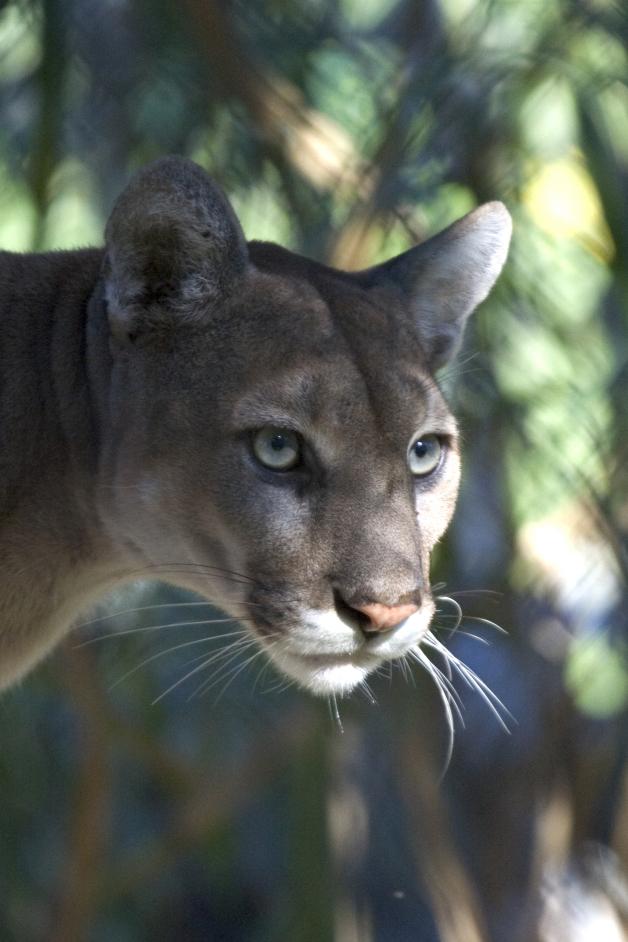
\includegraphics[fig.height=5.5cm,keepaspectratio]{figs/panther1}
% 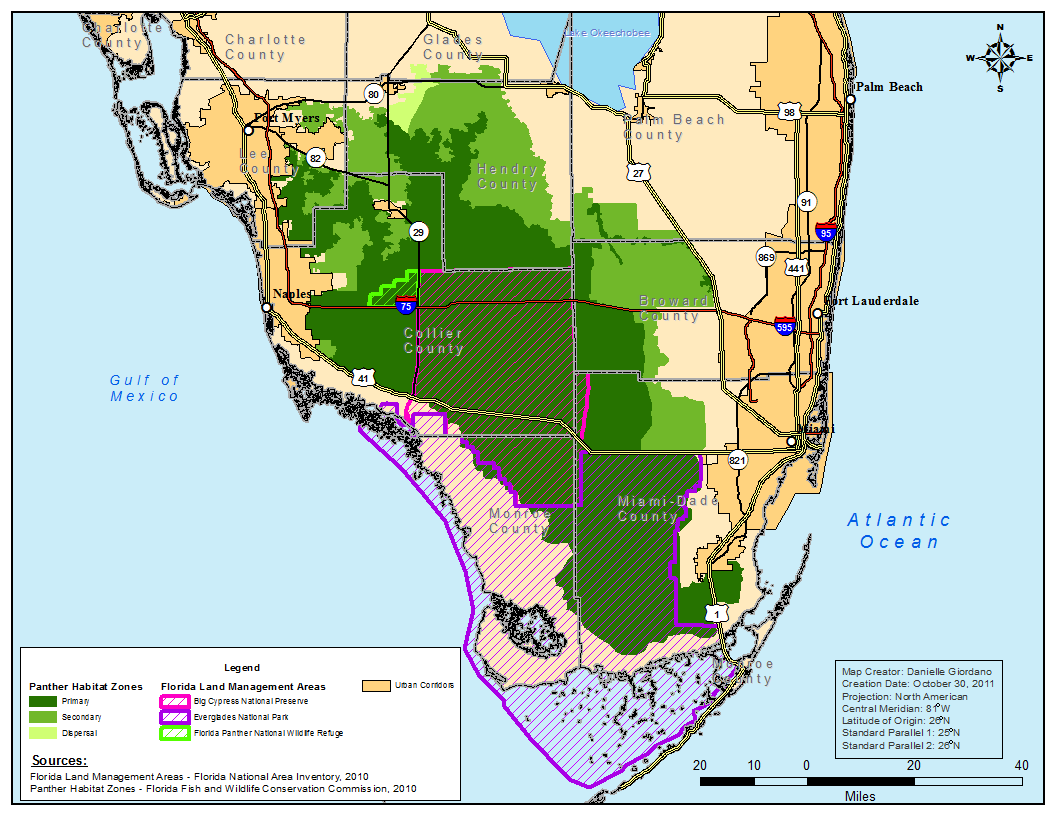
\includegraphics[fig.height=5.5cm,keepaspectratio]{figs/FloridaPantherHabitat}
 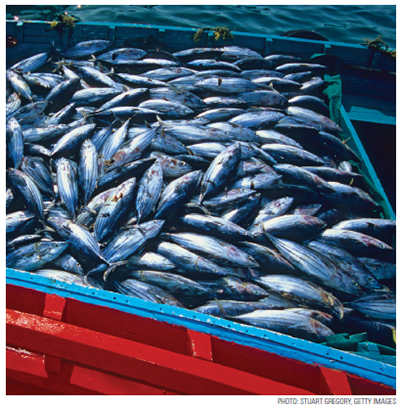
\includegraphics[height=6.5cm,keepaspectratio]{figs/tuna}
  \end{center}
\end{frame}




\begin{frame}
  \frametitle{Issues}
  {\flushleft Larkin, P.A. 1977. An epitaph for the concept of maximum
    sustained yield. Transactions of the American Fisheries Society 106: 1-11. \par}
  \pause
  \begin{itemize}%[<+->]
    \item Same assumptions as logistic growth model
      \begin{itemize}
        \item<3-> K is constant
        \item<3-> No age/sex/individual variation
        \item<3-> No stochasticity
      \end{itemize}
    \item<4-> Ecosystem impacts of reducing a population
      to half its carrying capacity?
    \item<5-> Evolutionary consequences?
%      \url{http://www.npr.org/templates/story/story.php?storyId=5434698}
  \end{itemize}
%  \pause
\end{frame}





\section{Compensatory mortality}


% Where is the density-dependence occuring? Is it in reproduction or
% survival or both??


% Back to the mechanisms


\begin{frame}
  \frametitle{Compensatory mortality}
  \large
  {\bf Additive vs. compensatory mortality}
  \begin{itemize}[<+->]
    \item One possible mechanism giving rise to logistic growth is
      density-dependence in survival
    \item For example, if population size is reduced, survival of the
      remaining individuals might increase
    \item If harvest is compensated for by improved survival, harvest
      is a form of \alert{\bf compensatory mortality}
    \item However, if harvest is not compensated for by improved
      survival, harvest is a form of \alert{\bf additive mortality}
  \end{itemize}
  \vfill
  \uncover<5->{
%  When setting harvest regulations, managers need to know if harvest
%  mortality is compensatory or additive.
    If harvest mortality is additive, extra caution is needed
    to ensure that harvest doesn't cause long-term population
    declines. \\
  }
\end{frame}



\begin{frame}
  \frametitle{Compensatory mortality example}
  \large
%  \begin{itemize}[<+->]
%    \item
  Suppose a population of 100 white-tailed deer is subjected to
  harvest \\
%    \item
  \pause \vfill
  Harvest takes place prior to any natural mortality \\
%    \item
  \pause \vfill
  Natural mortality occurs in a density dependent fashion,
  such that survival probability ($S$) declines as $N$ increases. \\
%    \item
  \pause \vfill
  A simple model is $S = \beta_0 - \beta1 \times N$ \\
  \pause \vfill
%    \item
  Let's assume $\beta_0 = 0.8$ and $\beta_1 = 0.005$, so
  $S = 0.8 - 0.005 \times N$
%  \end{itemize}
\end{frame}



\begin{frame}[fragile]
  \frametitle{Individual survival vs. population size}
%  $\phi = 0.8333 - 0.005556\times N$
%  \vspace{-0.5cm}

\centering
\includegraphics[width=\textwidth]{figure/phi1-1} \\
\end{frame}



% Break into teams and answer these questions. I will choose who presents
% OR, do this in socrativ


\begin{frame}
  \frametitle{$S = 0.8 - 0.005 \times N$}
%  \large
  \begin{itemize}[<+->]
    \small
    \item If 20 individuals are harvested, what is $S$ for
      remaining individuals?
    \item How many individuals will remain at the end of the year?
    \item How many would remain at the end of the year if no hunting
      occurred?
  \end{itemize}
  \begin{center}
    \includegraphics[width=0.7\textwidth]{figure/phi1-1}
  \end{center}
\end{frame}




\begin{frame}
  \frametitle{Overall survival vs. harvest rate}
  The overall survival rate ($\bar{S}$) is product of survival
  throughout the hunting season ($1-h$) and survial after the hunting
  season
  \Large
  \[
    \bar{S} = (1-h)(\beta_0 - \beta_1 (N - Nh))
  \]
\end{frame}


\begin{frame}[fragile]
  \frametitle{Overall survival vs. harvest rate}
  \vspace{-0.5cm}

\begin{center}
  \includegraphics[width=0.8\textwidth]{figure/phibar-1}
\end{center}
\pause
%\vfill
\small
{\bf Conclusion}: Because harvest mortality is compensatory, the
harvest rate ($h$) can be as high as 0.2 without negatively impacting
overall survival.
\end{frame}


%This curve of compensation is relatively flat for quite a range of
%harvest rates, because the natural survival rate compensates for the
%increase in harvest rate by increasing because of the decreasing
%number of animals in the population


\begin{frame}
  \frametitle{Summary}
%  \large
  {\bf Key points}
  \begin{itemize}
    \item If growth is geometric, sustainable harvest occurs when $h=r$
    \item If growth is logisitic, maximum sustainable yield occurs at $N=K/2$
    \item If survival is density-dependent, harvest mortality can be
      compensated for by increased survival of remaining individuals
      (up to a point)
    \item If mortality is additive, extra caution is needed
      because harvest is adding to natural mortality without any
      compensation
    \item Managers need to understand population dynamics when setting
      harvest regulations
  \end{itemize}
\end{frame}



\begin{frame}
  \frametitle{Assignment}
  \huge \centering
  Read pages 22--25 in Conroy and Carroll
\end{frame}




%\section{Case study}




\end{document}
